%%%%%%%%%%%%%%%%%%%%%%%%%%%%%%
\chapter{Background}

In this chapter, details regarding the simulation theory are gone over.  

%%%%%%%%%%%%%%%%%%%%%%%%%%%%%%
\section{Reactor Analysis}

What its all about

%%%%%%%%%%%%%%%%%%%%%%%%%%%%%%
\subsection{History}

The Monte Carlo method is not a new way to simulate nuclear reactors (or any particle transport problem for that matter) and in it's modern form dates back to 1940 when XXX invented the approach while working on the Manhattan Project[cite]. Uncle in Monaco...  During this time, Henry Metropolis and John Von Neumann...[cite]  Although this may be disputed by some people since is was rumored that Enrico Fermi was basically doing small scale simulations of this kind in his head trying to get the Chicago Pile critical [cite].


%%%%%%%%%%%%%%%%%%%%%%%%%%%%%%
\subsection{Nuclear Interactions}

The core of a Monte Carlo simulation is explicitly modeling the individual interactions the neutron undergoes as it moves through matter.  At the highest level, these reactions can be broken down into two categories, elastic reactions and inelastic reactions.  Elastic reactions are those where both momentum and kinetic energy are conserved, i.e. ones where any energy the neutron loses is given to the target nucleus.  Inelastic reactions are those that conserve momentum but do not conserve kinetic energy, i.e. ones where the kinetic energy of the particles can be converted to a vibrational mode of the target nucleus, etc.  These reactions are further divided by the number and type of secondary particles they produce.  Reactions that produce no secondary neutrons are called ``disappearance'' reactions since the neutron effectively disappears, reactions that produce a single neutron are typically called scattering reactions since they effectively change the incoming neutron's energy and direction, and reaction the produce more than one particle are simply called ``secondary-producing'' reactions. Table \ref{nuc_reaction_summary} show a summary of the reaction classifications, and it can be seen that elastic scattering is the only elastic reaction.   potential scattering vs compund nucleus.

\begin{table}[h]
\centering
\caption{Summary matrix of how neutron reactions are classified.}
\label{nuc_reaction_summary}
\begin{tabular}{| l | c | c | c |}
\multicolumn{4}{c}{Number of Secondaries} \\
\hline
  & 0 & 1 & $>$1 \\
 \hline
 Elastic & & Elastic Scatter & \\
 \hline
 Inelastic & Disappearance & Inelastic Scatter & Secondary-Producing \\
\hline
\end{tabular}
\end{table}

The probabilities for individual reactions occurring are expressed in terms of cross sections.  In simple terms, nuclear cross sections are like a geometric cross sections -they represent the ``size'' of the target nucleus for a particular reaction.  The classical analogy is that if neutrons and nuclei are hard spheres, and neutrons are randomly shot through a material, more neutrons will hit the larger targets than the smaller ones.  Cross sections are also expressed in units of area, the ``barn,'' which is $10^{-24}$ cm$^2$.  This unit was coined by Baker and Holloway while performing scattering experiments with uranium since ``a cross section of $10^{-24}$ cm$^2$ for nuclear purposes was really as big as a barn''\cite{LAMS523}.  Of course, nuclear cross sections have no literal meaning in terms of the actual sizes of the nuclei, they only represent the likelihood of a particular reaction occurring.  Working from the macroscopic scale, which is where measurements are taken, a \emph{macroscopic cross section}, represented by greek capital sigma ($\Sigma$), is the probability of a reaction happening within an infinitesimal distance d$x$.  With this parameter, we can write down an equation that describes the survival probability of a group of particles.  Describing a group is necessary since the dimension x is \emph{continuous}.  Given a particle packet containing N particles and $\Sigma$, their interaction probability over $d$x, the change the population over $d$x is the product of the population N and the interaction probability, as show in \eqref{pop_diff}.

\begin{equation}
\frac{d\mathrm{N}}{d\mathrm{x}} = - \Sigma \mathrm{N}
\label{pop_diff}
\end{equation}

Integrating \ref{pop_diff} over an interval yields an expression for the number of \emph{non-interacting} particles left in a packet after crossing that interval.  Dividing the surviving number by the initial gives a dimensionless expression for the non-interaction probability, P$_\mathrm{NI}$, over the interval x$_1$ as shown in \eqref{pop_NI}.

\begin{equation}
\mathrm{P}_\mathrm{NI} = \frac{\mathrm{N}}{\mathrm{N}_0} = \mathrm{e}^{- \Sigma \mathrm{x}_1}
\label{pop_NI}
\end{equation}

\begin{equation}
\Sigma = \frac{ - \mathrm{ln}(    \mathrm{I} / \mathrm{I}_0  )  }  {\mathrm{x}_1}
\label{pop_beam}
\end{equation}

Since these expressions also apply to beam intensity, they can be used to measure the cross sections for materials by rearranging the equations into the form shown in \eqref{pop_beam}.  If the source intensity, the exiting intensity, and the material thickness are all known, the macroscopic cross section for that material can be determined.  On a microscopic level, however, the neutron interaction probabilities only depend on the type of nucleus, not the aggregate material.  To correct for this, the measured macroscopic cross section can be divided by the number density of nuclei in the material to give the microscopic cross section, $\sigma$, which is material-independent and only depends on the isotope.  In \eqref{micro_exp}, N represents the number density in units of cm$^{-3}$, $\rho$ represents the material density in terms of g*cm$^{-3}$, and M represents the nuclear mass in g.  The microscopic cross section has units of barns, and is what is given in nuclear data files.  They are more general since they are not material-dependent and can be summed into a total material macroscopic cross section by weighting individual microscopic cross sections with the number density of an isotope in a material, as show in \eqref{material_sum_xs}.  In this expression, $f_\mathrm{i}$ is the atomic fraction of isotope i in the material.

\begin{equation}
\Sigma = N \sigma = \frac{\rho}{M} \sigma
\label{micro_exp}
\end{equation}

\begin{equation}
\sum_{\mathrm{i}=1}^{\mathrm{N}_\mathrm{isotopes}} f_\mathrm{i} =1
\label{fraction_norm}
\end{equation}

\begin{equation}
\Sigma_{\mathrm{material}} = \mathrm{N}_1 \sigma_1 +  \mathrm{N}_2 \sigma_2 + \mathrm{N}_3 \sigma_3+ ... = \sum_{\mathrm{i}=1}^{\mathrm{N}_\mathrm{isotopes}} \mathrm{N}_\mathrm{i} \sigma_\mathrm{i} = \rho\frac{\sum_{\mathrm{i}=1}^{\mathrm{N}_\mathrm{isotopes}} f_\mathrm{i}\sigma_\mathrm{i} } { \sum_{\mathrm{i}=1}^{\mathrm{N}_\mathrm{isotopes}} f_\mathrm{i} \mathrm{M}_\mathrm{i}}
\label{material_sum_xs}
\end{equation}

The above expressions do not take energy into account, so they are assumed to be at a single energy.  Using such simple expressions to determine the cross section of an isotope would only be valid with the use of a very, very precisely mono-energetic beam.  The quantum mechanical details that go into cross sections can cause them to depend strongly on the energy (or velocity) of the neutron and the target nucleus.  Many nuclides have resonances where the interactions probability spikes to very large values.  This typically happens when the incoming energy is exactly that of an energy level of the resultant compound nucleus \cite{duderstadt}.   Figure \ref{xs_e_dependence_li} shows the energy dependence of various reactions type in lithium-6 and Figure \ref{xs_e_dependence_u} shows additional reactions in uranium-235.  

\begin{figure}[h]
  \label{xs_e_dependence_li}
  \centering
    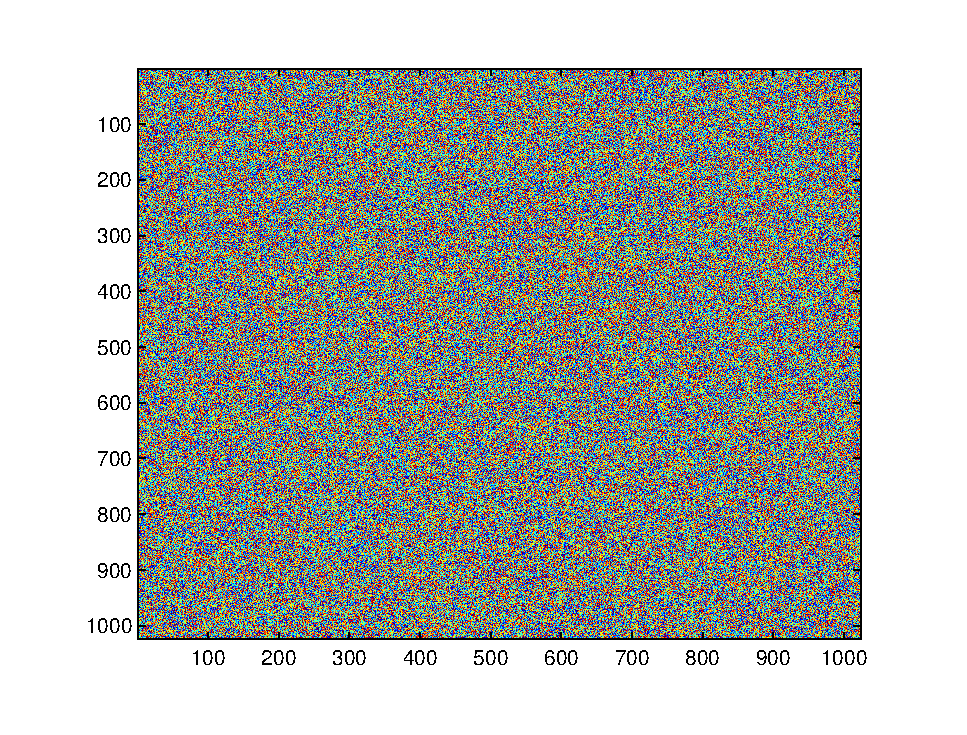
\includegraphics[width=0.85\textwidth]{xs/noise.eps}
     \caption{The energy dependence of some reactions in lithium-6.}
\end{figure}

\begin{figure}[h]
  \label{xs_e_dependence_u}
  \centering
    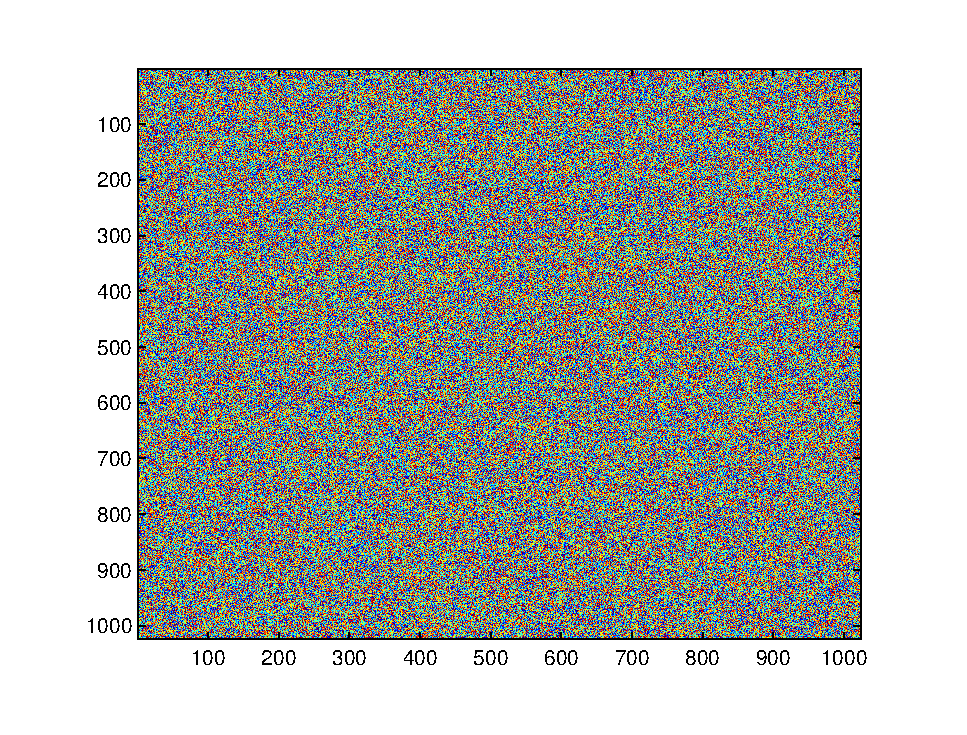
\includegraphics[width=0.85\textwidth]{xs/noise.eps}
    \caption{The energy dependence of some reactions in uranium-235.}
\end{figure}

It is important to note the complexity shown in uranium-235.  The strong energy dependence and lack of smoothness in regions. Cross section behavior, 1/v


\subsubsection{Elastic Scattering}

Elastic scattering conserves both the momentum and the kinetic energy of the reacting particles. 


\begin{equation}
\end{equation}

 Often, the energy of the neutron is much larger than that of the nucleus it is scattering off of, so the target velocity can be set to



\subsubsection{Inelastic Level Scattering}


\begin{equation}
\end{equation}

\subsubsection{Inelastic Continuum Scattering}

\begin{equation}
\end{equation}

\subsubsection{Fission}

\begin{equation}
\end{equation}

fission

\subsubsection{Other Inelastic Secondary-Producing Reactions}

\begin{equation}
\end{equation}

n,2n and n,alpha/n

\subsubsection{Disappearance Reactions}

radiative capture - n,a etc

%%%%%%%%%%%%%%%%%%%%%%%%%%%%%%
\subsection{Temperature Effects}

thermal motion, thermal peak

doppler



%%%%%%%%%%%%%%%%%%%%%%%%%%%%%%
\subsection{Nuclear Data}

it's all about the data




%%%%%%%%%%%%%%%%%%%%%%%%%%%%%%
\subsection{Neutron Transport}

NTE

\begin{equation}
\end{equation}

\subsection{Discrete Methods}

Diffusion, SN

drawbacks, limitations

\subsection{Monte Carlo}

instead of the neutron population being continuous and the spatial and energy dimensions discretized (and integrating along them), we make the population discrete (and integrate over it) and leave the other dimensions continuous! 

equations and derivations and such

scaling

advantages

drawbacks and limitations

%%%%%%%%%%%%%%%%%%%%%%%%%%%%%%

\section{GPUs}

Part of the reason GPUs are able to perform efficiently is do to their reliance on single instruction, multiple data (SIMD) execution.  This execution method uses the same instructions carried out over multiple pieces of data at the same time.  This reduces the amount of power used in control and therefore more math can be done per watt [citation definitely needed].  The GPU programming model abstracts SIMD execution by using threads, which can be thought of in the traditional sense . There are some tradeoffs, however, including limited on-board memory (currently 12 GB), limited cache and control space, and requiring data parallelism for full utilization.

Since all threads in a GPU thread block must execute the same instructions, having conditional statements based on random numbers can cause threads to be serialized, leading to resource under-utilization.  For example, in particle transport where a particle history is assigned to each thread, thread divergence mainly arises through particles undergoing different reactions based on the results of cross-section sampling.  Also, GPUs have even higher global memory latency than CPUs, up to 800 clock cycles on older cards, compared to about 50 cycles on a typical CPU.  It is also important to remember than GPUs are clocked much slower than CPUs, so the memory latency performance issue is even greater [5, 7]. 

another brief introduction.  

advantages

pitfalls, weaknesses

\subsection{Supercomputing}

how and why they came to be used for supercomputing.

\subsection{Architecture}

SIMD, threads

\subsection{Memory}

speed, levels, etc.  limitations 

\subsection{CUDA}

kernels

%%%%%%%%%%%%%%%%%%%%%%%%%%%%%%

\section{Previous Works}

talk about the work that other people did

\section{Preliminary Studies}

all my prelim work to motivate this project

\subsection{2D Scattering Game}


\subsection{Ray Tracing with OptiX}

%%%%%%%%%%%%%%%%%%%%%%%%%%%%%%

\section{Scope in Detail}


